\documentclass[../main.tex]{subfiles}

\begin{document}
	
	\section*{Erklärung betreffend des selbstständigen Verfassens einer Projektarbeit an der School of Engineering}
	
	Mit der Abgabe dieser Projektarbeit versichert der/die Studierende, dass er/sie die Arbeit selbst-
	ständig und ohne fremde Hilfe verfasst hat. (Bei Gruppenarbeiten gelten die Leistungen der übrigen
	Gruppenmitglieder nicht als fremde Hilfe.)\vspace{5mm}
	
	Der/die unterzeichnende Studierende erklärt, dass alle zitierten Quellen (auch Internetseiten) im Text
	oder Anhang korrekt nachgewiesen sind, d.h. dass die Projektarbeit keine Plagiate enthält, also keine
	Teile, die teilweise oder vollständig aus einem fremden Text oder einer fremden Arbeit unter Vorgabe der
	eigenen Urheberschaft bzw. ohne Quellenangabe übernommen worden sind.\vspace{5mm}
	
	Bei Verfehlungen aller Art treten die Paragrafen 46 (Unredlichkeit und Verfahren bei Unredlichkeit) der
	ZHW Prüfungsordnung sowie die Bestimmungen der Disziplinarmassnahmen der Hochschulordnung in
	Kraft.\vspace{15mm}
	
	\noindent\begin{tabular}{@{}p{2.5in}p{2.5in}@{}}
		Ort, Datum                       & \dotfill\\
		\\
		Deniz Akca                       & \dotfill\\
		\\
		Dennis Bannerman                 & \dotfill\\
		\\
		Mike Iten                        & \dotfill\\
	\end{tabular} 
	
	\newpage
	\section{Abstract}
	Bei Aquaponics handelt es sich um den Kreislauf zwischen Aquakultur und Hydroponik. Aquakultur steht für die Zucht von Wassertieren in einem Becken und Hydroponiks steht für die Pflanzliche Kultivierung. \\
	
	
	\begin{figure}[H]
		\centering
		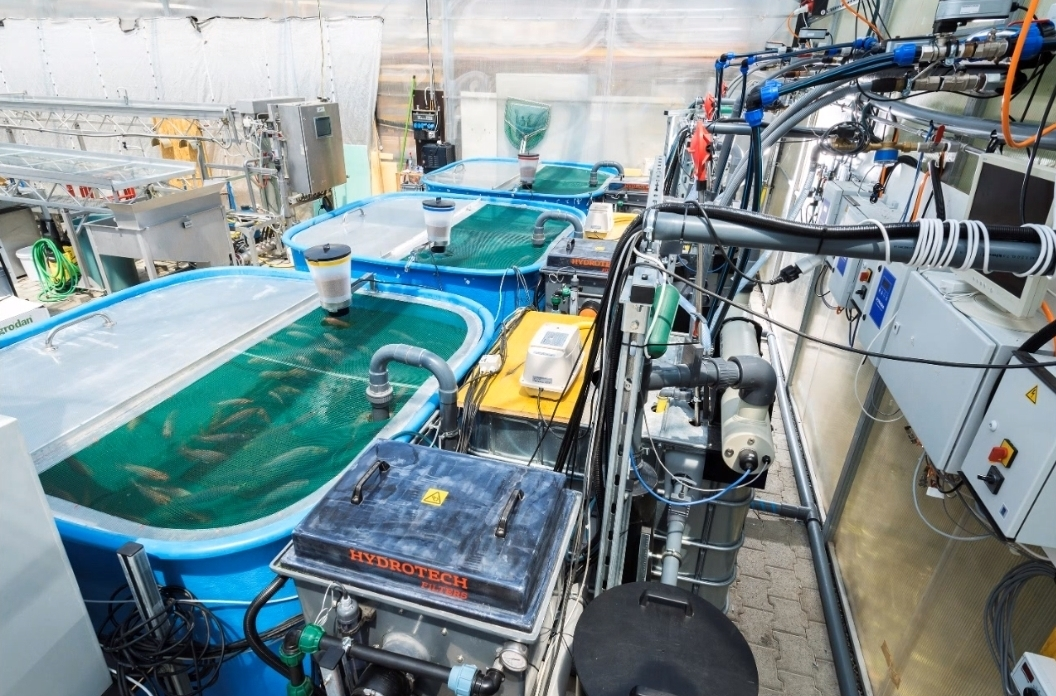
\includegraphics[scale=0.5]{Aquaponics_Tank}
		\caption{Tank in Wädischwil}
		\label{fig:Aquaponics_Tank}
	\end{figure}
	\par \noindent
	Unsere Aufgabe ist die Überwachung der \gls{sensor} in den Systemen zu vereinfachen. \\
	
	\section{Einleitung}
	
	\subsection{Ausgangslage}
	Ein Aquaponics Projekt besteht bereits aus folgenden Komponenten. \gls{sensor} der Aquaponics Systeme, welche an \gls{sc1000} Geräten angeschlossen sind. \\
	Ein serieller Bus verknüpft alle \gls{sc1000} mit einem RasPi welches über eine Modbus-API die Sensordaten auf eine \gls{mysql} Datenbank ablegt. Diese Daten werden auf der Webseite dargestellt. \\
	Die Webseite, welche unter myaquaculturefarm.ch zu finden ist, wird auf hosttech.ch gehostet. \gls{hosttech} verwendet als Backend Technologie \gls{php}.\\
	Unsere Konfigurationsseite wird ebenfalls auf dieser \gls{domain} parallel zu den anderen Webseiten von ZHAW Life Sciences und Facility Management gehostet. \\
	Beim Backend sind wir gebunden was die Host-Firma uns zur Verfügung stellt, in diesem Falle wäre das \gls{php}.
	
	\begin{figure}[H]
		\centering
		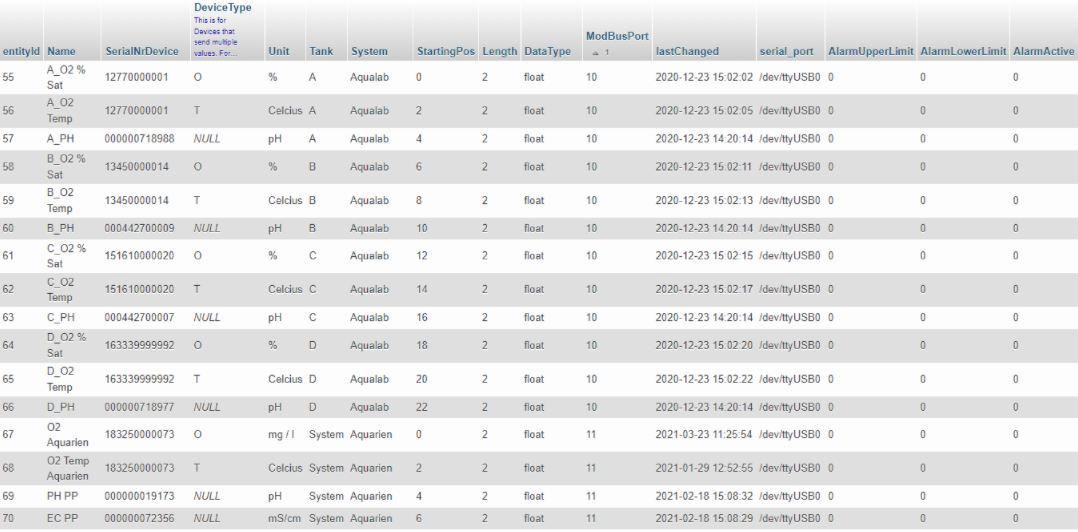
\includegraphics[scale=0.5]{Modbusentity}
		\caption{Modbusentity Tabelle}
		\label{fig:Modbusentity}
	\end{figure}
	\par \noindent
	Wie in der oberen Abbildung zu sehen ist werden die gesamten Sensorendaten in diese Tabelle eingespeist. Dadurch, dass es kein Interface gibt müssen die Daten jedesmal manuell in die Tabelle eingetragen werden. Falls es neue Tanks gibt benötigen sie eine neue Erkennungsnummer.  \\
	In der folgenden Abbildung werden die Daten geloggt um ein Archivierung älterer Daten zu ermöglichen.
	
	\begin{figure}[H]
		\centering
		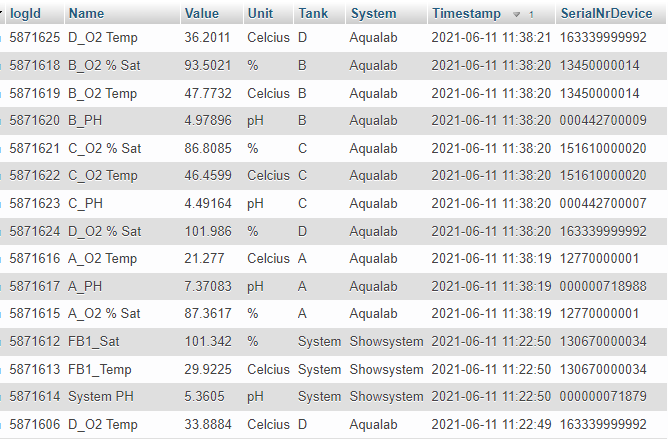
\includegraphics[scale=0.5]{Modbuslog}
		\caption{Modbuslog Tabelle}
		\label{fig:Modbuslog}
	\end{figure}
	\par \noindent	
	Um die Übersicht über die einzelnen Tanks zu wahren gibt es hier die Kolonnen Tank und Systeme, welche anzeigen woher die einzelnen Sensorendaten stammen.
	
	\subsection{Gesamtarchitektur}
	In den Becken befinden sich \gls{sensor} die verschiedene Messungen führen. Alle \gls{sensor} eines Systems hängen an einem \gls{sc1000} Gerät. Alle \gls{sc1000} Geräte sind mit dem Modbus verbunden. Über diesen Modbus holt sich das ein \gls{raspberrypi} alle Sensordaten von allen Systemen und logt und ladet diese hoch auf eine \gls{mysql} Datenbank. Dass das \gls{raspberrypi}i auch weiss an welcher Adresse auf dem Mobdus welcher \gls{sensor} abgefragt werden kann, werden die Konfigurationen aller Systeme innerhalb der \gls{mysql} Datenbank gespeichert.
	\begin{figure}[H]
		\centering
		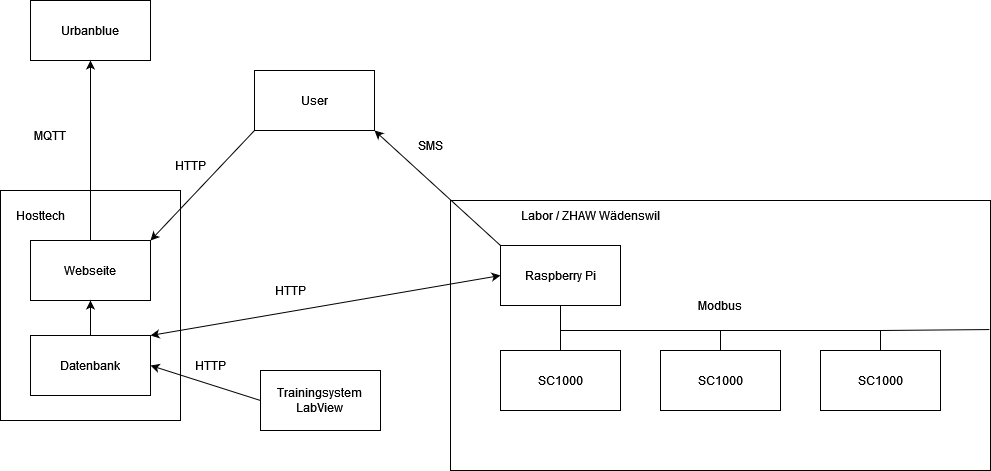
\includegraphics[scale=0.3]{pa_altes_system}
		\caption{Überblick aktuelles System}
		\label{fig:pa_altes_system}
	\end{figure}
	
	\subsection{Aufgabenstellung}
	Die Datenbank, in der die Sensordaten geloggt werden, besteht aus zwei Tabellen. In einer der Tabellen werden die \gls{sensor} eingetragen, die sich in den Systemen befinden und in der zweiten Tabelle werden die Sensordaten abgespeichert und mit dem jeweiligen \gls{sensor} verknüpft. \\
	\\	
	Das Bearbeiten dieser Zuordnungstabelle ist für die Mitarbeiter/Studierende der ZHAW Life Sciences und Facility Management mit dem von \gls{hosttech} gegebenen Tool \gls{phpmyadmin} nicht verständlich. Zusätzlich müssen spezifische Werte eingegeben werden die einen Informatik Laien nicht bekannt sind, welches zu inkorrekte Angabe von Daten führen kann, welches wiederum zu einem Durcheinander in der \gls{logtabelle} führt. 
	Das \gls{phpmyadmin} Tool ist ebenfalls nur per Verwaltungsseite der \gls{hosttech} \gls{domain} erreichbar welches eine zusätzliche Hürde darstellt.
	
	\subsection{Zielsetzung}
	Um die \gls{zuordnungstabelle} einfacher zu bearbeiten, soll der Ablauf abgeändert werden. Als Lösung stellen wir eine \gls{rest} Schnittstelle zur Verfügung über welche die Tabelle mit wenigen Handgriffen verändert werden kann. 
	Diese soll übersichtlich und einfach zu bedienen sein. Damit die Schnittstelle zu jeder Zeit erreichbar ist soll sie gehostet werden.
\end{document}